% Options for packages loaded elsewhere
\PassOptionsToPackage{unicode}{hyperref}
\PassOptionsToPackage{hyphens}{url}
\PassOptionsToPackage{dvipsnames,svgnames,x11names}{xcolor}
%
\documentclass[
  10pt,
]{article}
\usepackage{amsmath,amssymb}
\usepackage{iftex}
\ifPDFTeX
  \usepackage[T1]{fontenc}
  \usepackage[utf8]{inputenc}
  \usepackage{textcomp} % provide euro and other symbols
\else % if luatex or xetex
  \usepackage{unicode-math} % this also loads fontspec
  \defaultfontfeatures{Scale=MatchLowercase}
  \defaultfontfeatures[\rmfamily]{Ligatures=TeX,Scale=1}
\fi
\usepackage{lmodern}
\ifPDFTeX\else
  % xetex/luatex font selection
  \setmainfont[]{DejaVu Sans}
  \setmonofont[]{DejaVu Sans Mono}
  \setmathfont[]{DejaVu Sans}
\fi
% Use upquote if available, for straight quotes in verbatim environments
\IfFileExists{upquote.sty}{\usepackage{upquote}}{}
\IfFileExists{microtype.sty}{% use microtype if available
  \usepackage[]{microtype}
  \UseMicrotypeSet[protrusion]{basicmath} % disable protrusion for tt fonts
}{}
\makeatletter
\@ifundefined{KOMAClassName}{% if non-KOMA class
  \IfFileExists{parskip.sty}{%
    \usepackage{parskip}
  }{% else
    \setlength{\parindent}{0pt}
    \setlength{\parskip}{6pt plus 2pt minus 1pt}}
}{% if KOMA class
  \KOMAoptions{parskip=half}}
\makeatother
\usepackage{xcolor}
\usepackage[margin=2.2cm]{geometry}
\usepackage{color}
\usepackage{fancyvrb}
\newcommand{\VerbBar}{|}
\newcommand{\VERB}{\Verb[commandchars=\\\{\}]}
\DefineVerbatimEnvironment{Highlighting}{Verbatim}{commandchars=\\\{\}}
% Add ',fontsize=\small' for more characters per line
\newenvironment{Shaded}{}{}
\newcommand{\AlertTok}[1]{\textcolor[rgb]{1.00,0.00,0.00}{\textbf{#1}}}
\newcommand{\AnnotationTok}[1]{\textcolor[rgb]{0.38,0.63,0.69}{\textbf{\textit{#1}}}}
\newcommand{\AttributeTok}[1]{\textcolor[rgb]{0.49,0.56,0.16}{#1}}
\newcommand{\BaseNTok}[1]{\textcolor[rgb]{0.25,0.63,0.44}{#1}}
\newcommand{\BuiltInTok}[1]{\textcolor[rgb]{0.00,0.50,0.00}{#1}}
\newcommand{\CharTok}[1]{\textcolor[rgb]{0.25,0.44,0.63}{#1}}
\newcommand{\CommentTok}[1]{\textcolor[rgb]{0.38,0.63,0.69}{\textit{#1}}}
\newcommand{\CommentVarTok}[1]{\textcolor[rgb]{0.38,0.63,0.69}{\textbf{\textit{#1}}}}
\newcommand{\ConstantTok}[1]{\textcolor[rgb]{0.53,0.00,0.00}{#1}}
\newcommand{\ControlFlowTok}[1]{\textcolor[rgb]{0.00,0.44,0.13}{\textbf{#1}}}
\newcommand{\DataTypeTok}[1]{\textcolor[rgb]{0.56,0.13,0.00}{#1}}
\newcommand{\DecValTok}[1]{\textcolor[rgb]{0.25,0.63,0.44}{#1}}
\newcommand{\DocumentationTok}[1]{\textcolor[rgb]{0.73,0.13,0.13}{\textit{#1}}}
\newcommand{\ErrorTok}[1]{\textcolor[rgb]{1.00,0.00,0.00}{\textbf{#1}}}
\newcommand{\ExtensionTok}[1]{#1}
\newcommand{\FloatTok}[1]{\textcolor[rgb]{0.25,0.63,0.44}{#1}}
\newcommand{\FunctionTok}[1]{\textcolor[rgb]{0.02,0.16,0.49}{#1}}
\newcommand{\ImportTok}[1]{\textcolor[rgb]{0.00,0.50,0.00}{\textbf{#1}}}
\newcommand{\InformationTok}[1]{\textcolor[rgb]{0.38,0.63,0.69}{\textbf{\textit{#1}}}}
\newcommand{\KeywordTok}[1]{\textcolor[rgb]{0.00,0.44,0.13}{\textbf{#1}}}
\newcommand{\NormalTok}[1]{#1}
\newcommand{\OperatorTok}[1]{\textcolor[rgb]{0.40,0.40,0.40}{#1}}
\newcommand{\OtherTok}[1]{\textcolor[rgb]{0.00,0.44,0.13}{#1}}
\newcommand{\PreprocessorTok}[1]{\textcolor[rgb]{0.74,0.48,0.00}{#1}}
\newcommand{\RegionMarkerTok}[1]{#1}
\newcommand{\SpecialCharTok}[1]{\textcolor[rgb]{0.25,0.44,0.63}{#1}}
\newcommand{\SpecialStringTok}[1]{\textcolor[rgb]{0.73,0.40,0.53}{#1}}
\newcommand{\StringTok}[1]{\textcolor[rgb]{0.25,0.44,0.63}{#1}}
\newcommand{\VariableTok}[1]{\textcolor[rgb]{0.10,0.09,0.49}{#1}}
\newcommand{\VerbatimStringTok}[1]{\textcolor[rgb]{0.25,0.44,0.63}{#1}}
\newcommand{\WarningTok}[1]{\textcolor[rgb]{0.38,0.63,0.69}{\textbf{\textit{#1}}}}
\usepackage{longtable,booktabs,array}
\usepackage{calc} % for calculating minipage widths
% Correct order of tables after \paragraph or \subparagraph
\usepackage{etoolbox}
\makeatletter
\patchcmd\longtable{\par}{\if@noskipsec\mbox{}\fi\par}{}{}
\makeatother
% Allow footnotes in longtable head/foot
\IfFileExists{footnotehyper.sty}{\usepackage{footnotehyper}}{\usepackage{footnote}}
\makesavenoteenv{longtable}
\usepackage{graphicx}
\makeatletter
\def\maxwidth{\ifdim\Gin@nat@width>\linewidth\linewidth\else\Gin@nat@width\fi}
\def\maxheight{\ifdim\Gin@nat@height>\textheight\textheight\else\Gin@nat@height\fi}
\makeatother
% Scale images if necessary, so that they will not overflow the page
% margins by default, and it is still possible to overwrite the defaults
% using explicit options in \includegraphics[width, height, ...]{}
\setkeys{Gin}{width=\maxwidth,height=\maxheight,keepaspectratio}
% Set default figure placement to htbp
\makeatletter
\def\fps@figure{htbp}
\makeatother
\setlength{\emergencystretch}{3em} % prevent overfull lines
\providecommand{\tightlist}{%
  \setlength{\itemsep}{0pt}\setlength{\parskip}{0pt}}
\setcounter{secnumdepth}{-\maxdimen} % remove section numbering

\usepackage{xcolor}
\definecolor{plblue}{HTML}{1F3864}
\usepackage{sectsty}
\allsectionsfont{\sffamily\color{plblue}}
\usepackage{fvextra}
\DefineVerbatimEnvironment{Highlighting}{Verbatim}{breaklines,commandchars=\\\{\},fontsize=\footnotesize}
\usepackage{etoolbox}
\AtBeginEnvironment{longtable}{\footnotesize}
\ifLuaTeX
  \usepackage{selnolig}  % disable illegal ligatures
\fi
\IfFileExists{bookmark.sty}{\usepackage{bookmark}}{\usepackage{hyperref}}
\IfFileExists{xurl.sty}{\usepackage{xurl}}{} % add URL line breaks if available
\urlstyle{same}
\hypersetup{
  colorlinks=true,
  linkcolor={Maroon},
  filecolor={Maroon},
  citecolor={Blue},
  urlcolor={Blue},
  pdfcreator={LaTeX via pandoc}}

\author{}
\date{}

\begin{document}

\hypertarget{document-1-circuit}{%
\section{Document 1: Circuit}\label{document-1-circuit}}

\textbf{Kit:} qae\_european 1.0.0 · \textbf{Scope:} what the circuit
computes, how, with which inputs and outputs, and how to reproduce every
number in the kit.

Companion documents: \href{benchmarks.md}{Document 2: Benchmarks} ·
\href{tests.md}{Document 3: Tests} · \href{../README.md}{User guide}.

\begin{center}\rule{0.5\linewidth}{0.5pt}\end{center}

\hypertarget{1-purpose}{%
\subsection{1. Purpose}\label{1-purpose}}

The kit prices a European call under Black-Scholes with
\textbf{amplitude estimation} on a quantum circuit simulator. The aim is
not to price this option (it has a closed form) but to provide the
smallest complete example of the method: loading a distribution,
encoding a payoff, estimating an amplitude, and validating the result
against classical references.

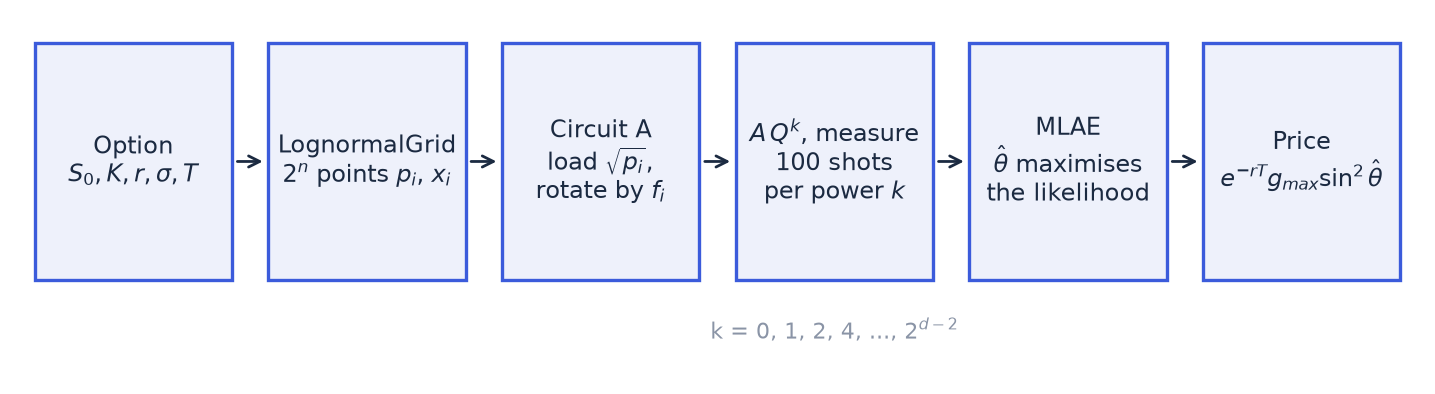
\includegraphics{img/pipeline.png}

\hypertarget{2-model-and-target}{%
\subsection{2. Model and target}\label{2-model-and-target}}

Under Black-Scholes, the terminal price is lognormal under the
risk-neutral measure:

ln S\_T \textasciitilde{} N(μ, s²), μ = ln S₀ + (r − σ²/2) T, s = σ √T.

The target is the call price C = e\^{}(−rT) E{[}max(S\_T − K, 0){]}. The
underlying pays no dividend. Inputs are validated in \texttt{Option}
(\texttt{option.py}): S₀, K, σ, T must be positive and finite; r must be
finite and may be negative.

\hypertarget{3-discretisation-gridpy}{%
\subsection{\texorpdfstring{3. Discretisation
(\texttt{grid.py})}{3. Discretisation (grid.py)}}\label{3-discretisation-gridpy}}

A circuit on n qubits holds 2ⁿ basis states, so the distribution is
discretised on 2ⁿ points.

\begin{enumerate}
\def\labelenumi{\arabic{enumi}.}
\item
  \textbf{Range.} The log-price interval {[}μ − w·s, μ + w·s{]} is cut
  into 2ⁿ bins of equal width in log-price, with w = 4 by default
  (\texttt{width}).
\item
  \textbf{Probabilities.} Bin i carries p\_i = Φ(z\_\{i+1\}) − Φ(z\_i),
  with z the standardised edges. The probabilities are renormalised to
  sum to 1. The mass outside the range, 2Φ(−4) ≈ 6.3·10⁻⁵, is spread
  proportionally over the bins.
\item
  \textbf{Representative prices.} Bin i is represented by the
  conditional mean of S\_T in the bin, which has a closed form for a
  lognormal:

  x\_i = E{[}S\_T \textbar{} S\_T in bin i{]} = e\^{}(μ + s²/2) ·
  {[}Φ(z\_\{i+1\} − s) − Φ(z\_i − s){]} / p\_i.

  Using conditional means rather than bin midpoints makes the
  discretised forward match the true forward, up to the truncated mass.
\end{enumerate}

The \textbf{grid price} is P\_grid = e\^{}(−rT) Σ\_i p\_i max(x\_i − K,
0). It is the exact target of the circuit. Its gap to Black-Scholes is
the \textbf{discretisation bias}, which depends only on n, w and the
option, not on any sampling. The bias falls as n grows.

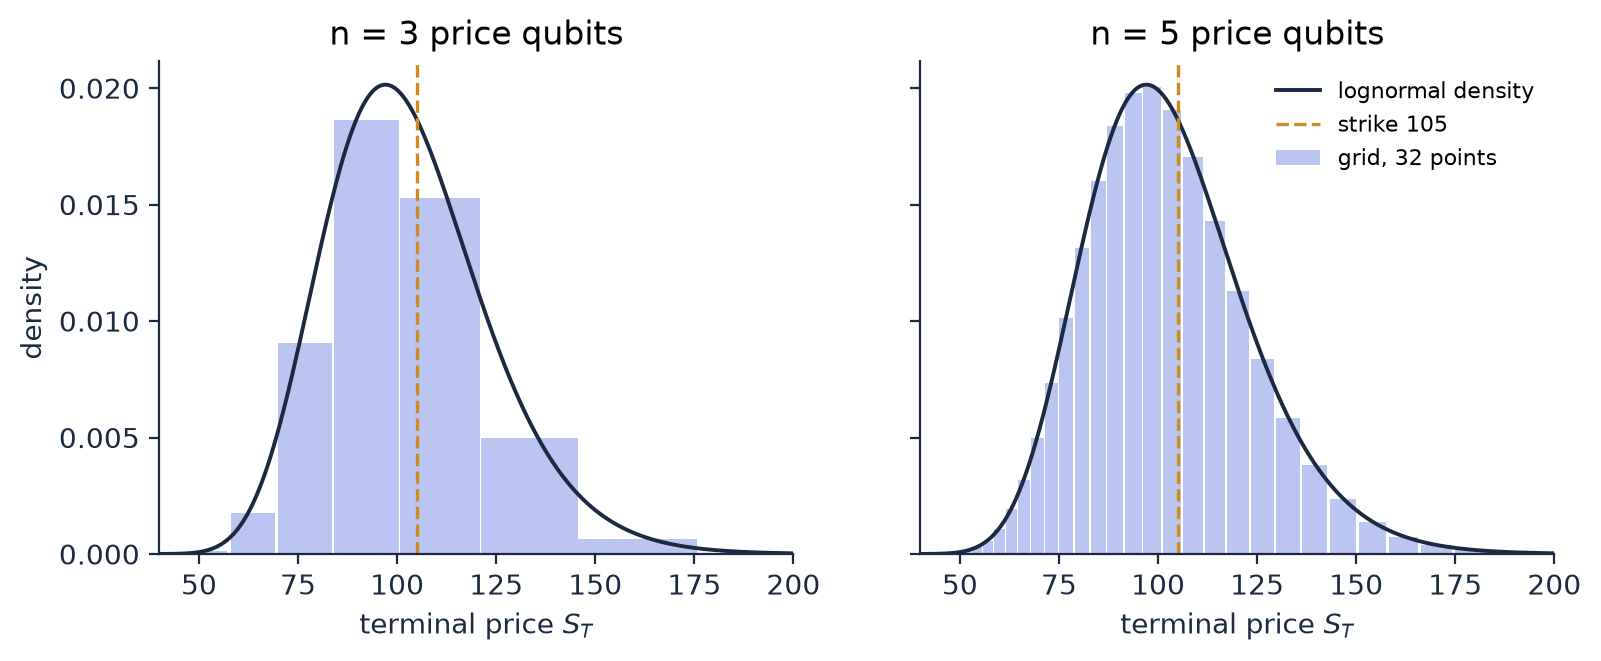
\includegraphics{img/discretisation.png}

\emph{Reference option of the guide: S₀ = 100, K = 105, r = 3\%, σ =
20\%, T = 1.}

\hypertarget{4-the-circuit-a-quantumpy}{%
\subsection{\texorpdfstring{4. The circuit A
(\texttt{quantum.py})}{4. The circuit A (quantum.py)}}\label{4-the-circuit-a-quantumpy}}

The circuit acts on \textbf{n + 1 qubits}:

\begin{itemize}
\tightlist
\item
  qubits 0 to n − 1: the \textbf{price register}. Basis state
  \textbar i⟩ stands for grid point i, with qubit 0 the least
  significant bit (Qiskit\textquotesingle s convention).
\item
  qubit n: the \textbf{objective qubit}.
\end{itemize}

\textbf{Block 1: load the distribution.} \texttt{StatePreparation}
prepares Σ\_i √p\_i \textbar i⟩ on the price register. This is exact
loading: Qiskit synthesises a circuit for an arbitrary state.

\textbf{Block 2: encode the payoff.} With g\_i = max(x\_i − K, 0) and
g\_max = max\_i g\_i, the normalised payoffs are f\_i = g\_i / g\_max,
in {[}0, 1{]}. For each grid point with f\_i \textgreater{} 0, a
rotation RY(θ\_i) with θ\_i = 2 arcsin(√f\_i) is applied to the
objective qubit, controlled on the price register being exactly
\textbar i⟩. The control on \textbar i⟩ is built with X gates on the
price qubits where bit i is 0, before and after a rotation controlled on
all n price qubits. Grid points out of the money get no rotation.

After A, the state is Σ\_i √p\_i \textbar i⟩ ⊗ (√(1 − f\_i) \textbar0⟩ +
√f\_i \textbar1⟩). The probability of measuring the objective qubit in
state 1 is therefore

a = Σ\_i p\_i f\_i = E\_grid{[}g{]} / g\_max, and P\_grid = e\^{}(−rT) ·
g\_max · a.

The kit writes a = sin²θ with θ in {[}0, π/2{]}. If every grid point is
out of the money (g\_max = 0), the option is \textbf{worthless on the
grid}: the price is exactly 0 and nothing is estimated.

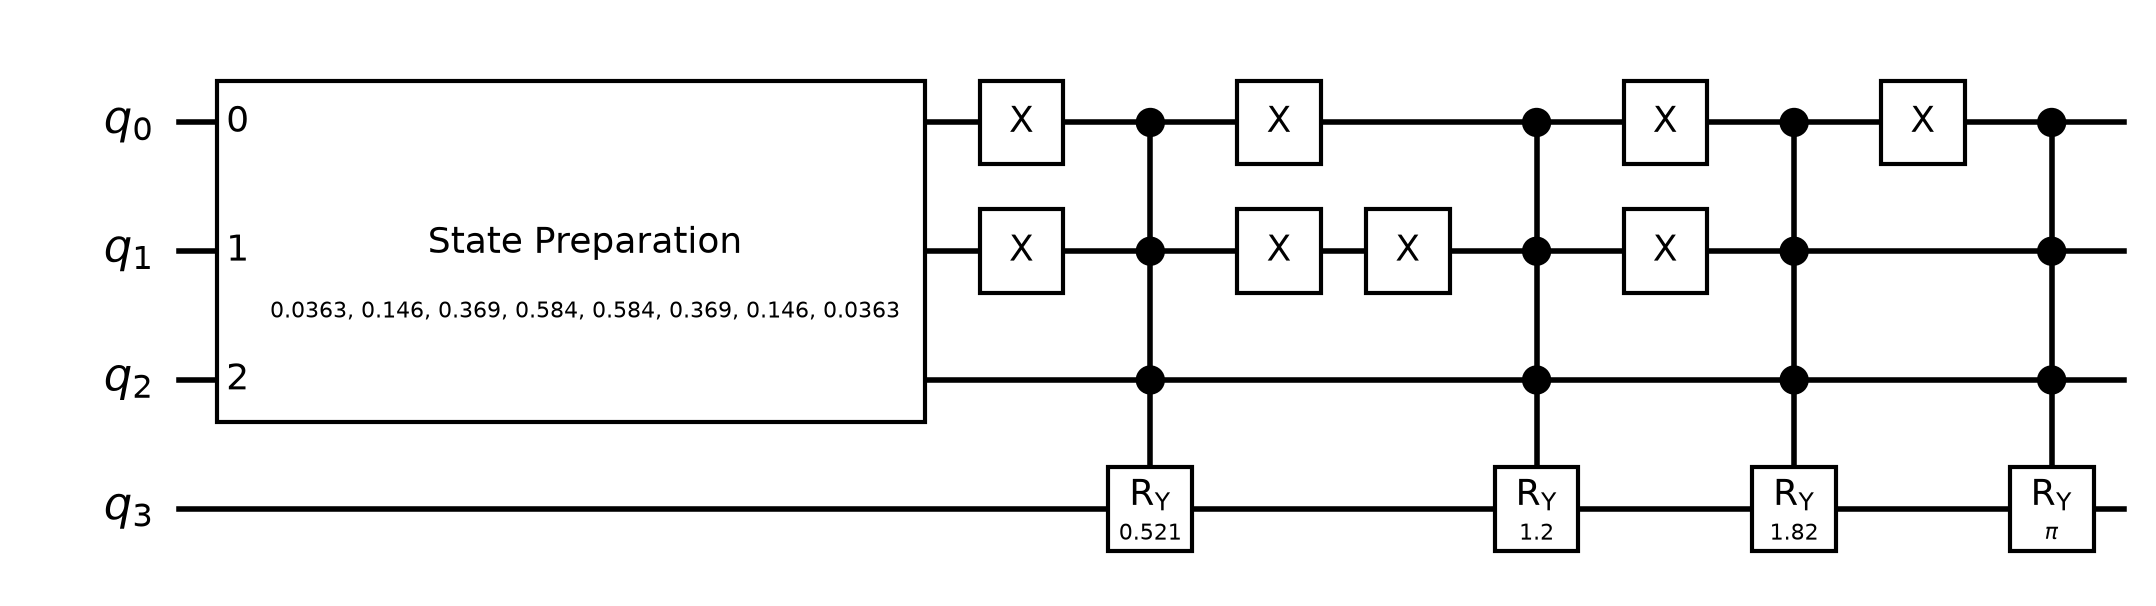
\includegraphics{img/circuit_a_3qubits.png}

\emph{Four grid points are in the money, so A has four controlled
rotations. The last one is RY(π), since f = 1 at the largest payoff.}

\hypertarget{5-the-grover-operator-q}{%
\subsection{5. The Grover operator Q}\label{5-the-grover-operator-q}}

Q = A S₀ A† S\_χ, up to a global phase of π, where:

\begin{itemize}
\tightlist
\item
  S\_χ applies a phase −1 to states with the objective qubit in 1: a Z
  gate on qubit n.
\item
  S₀ applies a phase −1 to \textbar0\ldots0⟩. It is built as X on all
  qubits, a multi-controlled Z (H, multi-controlled X, H on qubit n),
  then X on all qubits.
\end{itemize}

Q rotates the state by 2θ in the plane spanned by the "good" and "bad"
components of A\textbar0⟩. After A and k applications of Q:

P(objective = 1) = sin²((2k + 1)θ).

The code sets the global phase of Q explicitly
(\texttt{global\_phase\ +=\ π}). It has no effect on measured
probabilities, but it makes Q equal to the textbook operator −A S₀ A†
S\_χ, which matters if Q is ever used under control.

\hypertarget{6-maximum-likelihood-amplitude-estimation-estimationpy}{%
\subsection{\texorpdfstring{6. Maximum-likelihood amplitude estimation
(\texttt{estimation.py})}{6. Maximum-likelihood amplitude estimation (estimation.py)}}\label{6-maximum-likelihood-amplitude-estimation-estimationpy}}

Phase estimation would need many controlled applications of Q. MLAE
(Suzuki et al., 2020) uses only plain circuits A Qᵏ and classical
post-processing.

\textbf{Ladder.} A ladder of depth d uses the Grover powers k ∈ \{0, 1,
2, 4, \ldots, 2\^{}(d−2)\}: d powers, the largest 2\^{}(d−2). Each
circuit A Qᵏ is measured 100 times (\texttt{shots}).

\textbf{Cost.} One measurement after k steps applies A once, then Q k
times. Each Q contains A and A†. The kit counts this as 2k + 1
applications of A (A† is counted as one application). The total cost of
a ladder is

N = shots × Σ\_k (2k + 1).

With 100 shots, depths 4 to 8 give N = 1,800, 3,500, 6,800, 13,300 and
26,200 calls.

\textbf{Estimator.} With h\_k ones out of \texttt{shots} at power k, θ
maximises the log-likelihood

L(θ) = Σ\_k {[} h\_k ln sin²((2k + 1)θ) + (shots − h\_k) ln cos²((2k +
1)θ) {]}.

It is maximised in two steps:

\begin{enumerate}
\def\labelenumi{\arabic{enumi}.}
\tightlist
\item
  a grid search over equally spaced points on {[}0, π/2{]}: at least
  4,001, and at least 200 per period of the most oscillating term (100 ×
  m\_max + 1 points, with m\_max = 2k\_max + 1);
\item
  a bounded scalar refinement (\texttt{scipy.optimize.minimize\_scalar},
  tolerance 10⁻¹²) within one grid step of each of the \textbf{5 highest
  local maxima} of the grid. The best refined point is kept.
\end{enumerate}

Probabilities are clipped to {[}10⁻¹⁵, 1 − 10⁻¹⁵{]} to avoid log(0). The
price estimate is e\^{}(−rT) g\_max sin²θ̂.

Why several candidates: when two peaks of the likelihood are nearly
tied, the grid can rank them in the wrong order, because it samples each
peak slightly off its top. Refining only the best grid point would then
return the lower peak. An earlier version did exactly that. An internal
review found it failed in about 1 draw in 200 at depth 8 and in every
draw at depth 14 on the widest scenario. It was corrected before the
campaign was re-run (Document 3, section 1.9). A unit test now compares
the estimator with a 400,001-point grid at depths 8 and 12, and
\texttt{docs/checks.py} does the same for every campaign configuration
with a mode error. \texttt{Ladder.exponential} accepts depths up to 16.

\textbf{Known limitation: mode errors.} L(θ) has several local maxima.
The higher powers make it oscillate quickly, while the low powers, which
only see a few shots each, are what tell those maxima apart.
Occasionally the noise in the low-power counts makes a wrong local
maximum the highest one. The estimate then lands about π/(2k\_max + 1)
away from the true θ. Such errors are rare but large.

This is a property of MLAE with an exponential ladder, not of the
optimiser: the estimate is the true global maximum of the likelihood
(\texttt{docs/checks.py}, results in Document 3, section 2.9). The
campaign keeps the published method unchanged, uses 50 draws per
configuration, and records the share of draws affected (Document 3,
sections 1.5 and 1.9).

\emph{How mode errors are counted.} A draw counts as a mode error when
\textbar θ̂ − θ\textbar{} \textgreater{} π/(2 m\_max), half the period of
the most oscillating term. Two consequences:

\begin{itemize}
\tightlist
\item
  The threshold is wide for short ladders (π/10 at depth 4). The absence
  of mode errors at low depth is partly a consequence of the definition.
\item
  A wrong peak lying closer to the true θ than the threshold would not
  be counted.
\end{itemize}

\hypertarget{7-simulating-the-measurements}{%
\subsection{7. Simulating the
measurements}\label{7-simulating-the-measurements}}

Two backends give the measurement probabilities. On a noise-free
simulator they are mathematically identical:

\begin{longtable}[]{@{}
  >{\raggedright\arraybackslash}p{(\columnwidth - 4\tabcolsep) * \real{0.1542}}
  >{\raggedright\arraybackslash}p{(\columnwidth - 4\tabcolsep) * \real{0.4718}}
  >{\raggedright\arraybackslash}p{(\columnwidth - 4\tabcolsep) * \real{0.3540}}@{}}
\toprule\noalign{}
\begin{minipage}[b]{\linewidth}\raggedright
Backend
\end{minipage} & \begin{minipage}[b]{\linewidth}\raggedright
How
\end{minipage} & \begin{minipage}[b]{\linewidth}\raggedright
Used for
\end{minipage} \\
\midrule\noalign{}
\endhead
\bottomrule\noalign{}
\endlastfoot
\texttt{statevector} & Builds A and Q in Qiskit and evolves the exact
statevector through A Qᵏ, then reads P(objective = 1). & Verification,
the user guide \\
\texttt{born} & Takes θ from the exact statevector of A, then uses P\_k
= sin²((2k + 1)θ). & The campaign (2.31 million amplitude-estimation
estimates) \\
\end{longtable}

In both cases, the measurement counts are then drawn as h\_k
\textasciitilde{} Binomial(shots, P\_k). This is exactly what a
noise-free sampler would return.

The \texttt{born} backend relies on the identity in section 5. It is
checked by full statevector simulation on 20 scenarios drawn at random,
for every number of qubits where the option is not worthless
(\texttt{qae-european\ verify}, hypothesis H0-b of Document 3):

\begin{itemize}
\tightlist
\item
  for n ≤ 5, powers up to 64, which covers the full ladder of depth 8;
\item
  for n = 6 and 7, powers up to 8, because simulation cost grows with
  the depth of A Qᵏ; plus the full ladder (powers up to 64) on the first
  of the 20 scenarios, so the largest circuits are also checked at the
  largest power the campaign uses.
\end{itemize}

The identity holds for any k: it follows from Q being a rotation.
Document 3 reports the outcome.

\hypertarget{8-circuit-size}{%
\subsection{8. Circuit size}\label{8-circuit-size}}

Compiled to a hardware-like gate set \{CX, RZ, SX, X\} with
Qiskit\textquotesingle s transpiler (optimisation level 1, seed 0), for
the reference option:

\begin{longtable}[]{@{}
  >{\raggedright\arraybackslash}p{(\columnwidth - 10\tabcolsep) * \real{0.1946}}
  >{\raggedright\arraybackslash}p{(\columnwidth - 10\tabcolsep) * \real{0.1274}}
  >{\raggedright\arraybackslash}p{(\columnwidth - 10\tabcolsep) * \real{0.1645}}
  >{\raggedright\arraybackslash}p{(\columnwidth - 10\tabcolsep) * \real{0.1645}}
  >{\raggedright\arraybackslash}p{(\columnwidth - 10\tabcolsep) * \real{0.1645}}
  >{\raggedright\arraybackslash}p{(\columnwidth - 10\tabcolsep) * \real{0.1645}}@{}}
\toprule\noalign{}
\begin{minipage}[b]{\linewidth}\raggedright
Price qubits n
\end{minipage} & \begin{minipage}[b]{\linewidth}\raggedright
Qubits
\end{minipage} & \begin{minipage}[b]{\linewidth}\raggedright
CNOTs in A
\end{minipage} & \begin{minipage}[b]{\linewidth}\raggedright
Depth of A
\end{minipage} & \begin{minipage}[b]{\linewidth}\raggedright
CNOTs in Q
\end{minipage} & \begin{minipage}[b]{\linewidth}\raggedright
Depth of Q
\end{minipage} \\
\midrule\noalign{}
\endhead
\bottomrule\noalign{}
\endlastfoot
3 & 4 & 84 & 290 & 182 & 606 \\
4 & 5 & 203 & 387 & 442 & 852 \\
5 & 6 & 626 & 1,037 & 1,334 & 2,178 \\
6 & 7 & 1,737 & 2,548 & 3,596 & 5,230 \\
7 & 8 & 5,000 & 12,155 & 10,170 & 24,491 \\
\end{longtable}

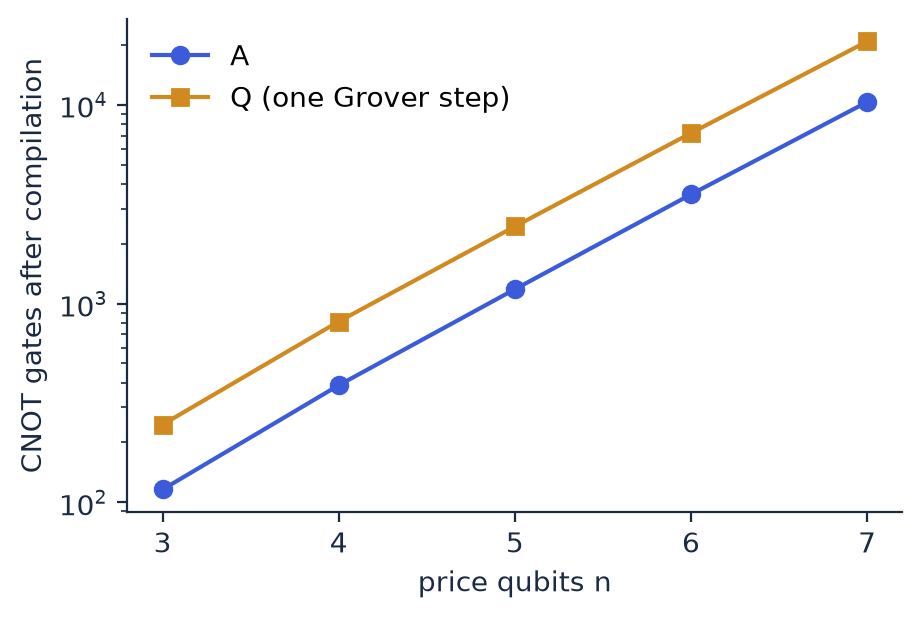
\includegraphics{img/circuit_size.png}

The count roughly triples per added qubit, i.e. it grows exponentially.
Both blocks are to blame:

\begin{itemize}
\tightlist
\item
  exact state preparation;
\item
  one multi-controlled rotation per in-the-money point.
\end{itemize}

At depth 8, one measurement at k = 64 applies Q 64 times: about 85,000
CNOTs for n = 5. That is far beyond today\textquotesingle s noisy
hardware, which is why the kit runs on a simulator. Efficient loading is
the open problem for practical use (Vazquez and Woerner, 2021;
Stamatopoulos and Zeng, 2024).

\hypertarget{9-inputs-and-outputs}{%
\subsection{9. Inputs and outputs}\label{9-inputs-and-outputs}}

\hypertarget{inputs}{%
\subsubsection{Inputs}\label{inputs}}

\begin{longtable}[]{@{}
  >{\raggedright\arraybackslash}p{(\columnwidth - 6\tabcolsep) * \real{0.2506}}
  >{\raggedright\arraybackslash}p{(\columnwidth - 6\tabcolsep) * \real{0.2102}}
  >{\raggedright\arraybackslash}p{(\columnwidth - 6\tabcolsep) * \real{0.2641}}
  >{\raggedright\arraybackslash}p{(\columnwidth - 6\tabcolsep) * \real{0.2552}}@{}}
\toprule\noalign{}
\begin{minipage}[b]{\linewidth}\raggedright
Input
\end{minipage} & \begin{minipage}[b]{\linewidth}\raggedright
Where
\end{minipage} & \begin{minipage}[b]{\linewidth}\raggedright
Type and range
\end{minipage} & \begin{minipage}[b]{\linewidth}\raggedright
Default
\end{minipage} \\
\midrule\noalign{}
\endhead
\bottomrule\noalign{}
\endlastfoot
spot, strike, vol, maturity & \texttt{Option} & float \textgreater{} 0 &
100, 105, 0.20, 1.0 \\
rate & \texttt{Option} & float, may be negative & 0.03 \\
n\_qubits & \texttt{LognormalGrid} & integer, 1 to 16 & --- (3 to 7 in
the campaign) \\
width & \texttt{LognormalGrid} & float \textgreater{} 0, standard
deviations & 4.0 \\
depth, shots & \texttt{Ladder.exponential} & integer ≥ 1 & --- , 100 \\
backend & \texttt{MaximumLikelihoodAE} & \texttt{"born"} or
\texttt{"statevector"} & \texttt{"born"} \\
seed / rng & all random methods & \texttt{numpy.random.Generator} &
--- \\
\end{longtable}

Invalid inputs raise \texttt{ValueError}. The kit uses \textbf{no
external data}: every input is a contract or market parameter given by
the user, or generated from the fixed scenario grid of the campaign.

\hypertarget{outputs}{%
\subsubsection{Outputs}\label{outputs}}

\begin{itemize}
\tightlist
\item
  \texttt{qae-european\ price}: JSON on standard output with the
  Black-Scholes, grid, exact-circuit, amplitude-estimation, Monte Carlo
  and quasi-Monte Carlo prices, and the number of calls. Prices are in
  the currency of the spot, discounted to today.
\item
  \texttt{qae-european\ verify}: \texttt{results/verification.json}, one
  record per (scenario, number of qubits): the largest power simulated,
  the largest absolute difference against sin²((2k + 1)θ), and the
  circuit-against-grid price difference.
\item
  \texttt{qae-european\ campaign}: \texttt{results/campaign.csv}, one
  row per (scenario, number of qubits, ladder depth). The columns are
  defined at the top of \texttt{src/qae\_european/campaign.py} and in
  Document 3, section 1.5. Floats are written at full double precision.
\end{itemize}

\hypertarget{10-environment-and-reproducibility}{%
\subsection{10. Environment and
reproducibility}\label{10-environment-and-reproducibility}}

\begin{longtable}[]{@{}
  >{\raggedright\arraybackslash}p{(\columnwidth - 2\tabcolsep) * \real{0.2884}}
  >{\raggedright\arraybackslash}p{(\columnwidth - 2\tabcolsep) * \real{0.6916}}@{}}
\toprule\noalign{}
\begin{minipage}[b]{\linewidth}\raggedright
Item
\end{minipage} & \begin{minipage}[b]{\linewidth}\raggedright
Value
\end{minipage} \\
\midrule\noalign{}
\endhead
\bottomrule\noalign{}
\endlastfoot
Python & 3.13.17 \\
Qiskit & 2.6.1 \\
NumPy & 2.5.4 \\
SciPy & 1.18.1 \\
Full pinned list & \texttt{requirements-lock.txt}, frozen in a clean
virtual environment \\
Operating system & Linux (x86-64, glibc 2.39) \\
CPU & 2-core Intel Xeon, 2.8 GHz \\
Quantum hardware & None: local noise-free simulation (Qiskit
\texttt{Statevector}) \\
Install & \texttt{pip\ install\ -r\ requirements-lock.txt} then
\texttt{pip\ install\ -\/-no-deps\ -e\ .} (user guide, section 1) \\
\end{longtable}

\textbf{Seeds.}

\begin{itemize}
\tightlist
\item
  The campaign derives every random stream from a master seed (20261103)
  and the indices of the scenario, number of qubits, ladder depth and
  method, through \texttt{numpy.random.SeedSequence}
  (\texttt{campaign.rng\_for}). Any row can be recomputed on its own
  (user guide, section 5).
\item
  The verification draws its 20 scenarios with the same master seed.
\item
  The transpiler in section 8 uses seed 0.
\end{itemize}

\textbf{Determinism.} In the frozen environment, results are bit-for-bit
reproducible:

\begin{itemize}
\tightlist
\item
  \textbf{Parallel runs:} they don\textquotesingle t change any value.
  Rows may appear in a different order in the CSV, because each
  scenario\textquotesingle s streams depend only on its own indices.
\item
  \textbf{Other library versions:} they may change the last digits. The
  order of random draws is fixed by NumPy\textquotesingle s
  \texttt{Generator} and SciPy\textquotesingle s Sobol implementation,
  which are stable within a major version but not guaranteed across
  them.
\end{itemize}

\textbf{Commands} (from \texttt{kits/qae\_european}):

\begin{Shaded}
\begin{Highlighting}[]
\ExtensionTok{pytest}\NormalTok{ tests                                   }\CommentTok{\# unit tests}
\ExtensionTok{qae{-}european}\NormalTok{ verify                            }\CommentTok{\# H0{-}b}
\ExtensionTok{qae{-}european}\NormalTok{ campaign }\AttributeTok{{-}{-}processes}\NormalTok{ 2            }\CommentTok{\# Document 3 campaign}
\ExtensionTok{python}\NormalTok{ docs/make\_figures.py                    }\CommentTok{\# figures of this document (needs the docs extra)}
\ExtensionTok{python}\NormalTok{ docs/analyse.py                         }\CommentTok{\# Document 3: criteria, summary.json and figures}
\ExtensionTok{python}\NormalTok{ docs/checks.py                          }\CommentTok{\# results/checks.json: state{-}preparation accuracy, MLAE global maximum}
\end{Highlighting}
\end{Shaded}

\hypertarget{11-limitations}{%
\subsection{11. Limitations}\label{11-limitations}}

\begin{itemize}
\tightlist
\item
  \textbf{Exact loading does not scale} (section 8). The kit
  demonstrates the method, not a practical pricer.
\item
  \textbf{Numerical precision of the synthesis.}
  Qiskit\textquotesingle s synthesis of the state preparation adds a
  floating-point error that grows with the number of qubits: about 10⁻¹³
  at n = 5, 10⁻¹¹ at n = 6 and 10⁻⁹ to 10⁻¹⁰ at n = 7 on the loaded
  probabilities (\texttt{docs/checks.py}). The circuit price then
  matches the grid price to a relative 10⁻⁸, not to machine precision.
  This is far below any statistical error, but it matters for
  exact-equality tests (Document 3, section 2.4).
\item
  \textbf{Noise-free simulation.} No hardware noise and no error
  mitigation. Real hardware would add errors that grow with circuit
  depth.
\item
  \textbf{The error is scaled by the largest payoff.} The price is read
  as e\^{}(−rT) g\_max a. With high volatility or long maturity, g\_max
  is far above the price: on the 5-year, 60\%-volatility at-the-money
  scenario, g\_max ≈ 7,100 for a price of about 49. The amplitude a is
  then small, and its error is magnified in the price. A narrower
  \texttt{width} reduces g\_max but increases the truncation bias. The
  default, 4 standard deviations, is a common choice and is not tuned
  per scenario.
\item
  \textbf{Mode errors of MLAE} (section 6).
\item
  \textbf{Call counts are not run times.} On a fault-tolerant machine,
  one application of A takes far longer than one Monte Carlo path on a
  classical processor. Published estimates of where a practical
  advantage could appear are in Chakrabarti et al. (2021) and
  Stamatopoulos and Zeng (2024).
\item
  \textbf{One product.} The construction applies to any payoff of S\_T
  that is non-negative on the grid (user guide, section 7).
  Path-dependent payoffs need a register per time step and are out of
  scope.
\end{itemize}

\hypertarget{references}{%
\subsection{References}\label{references}}

\begin{itemize}
\tightlist
\item
  Suzuki, Uno, Raymond, Tanaka, Onodera, Yamamoto, \emph{Amplitude
  estimation without phase estimation}, Quantum Information Processing
  19, 75 (2020).
  \href{https://arxiv.org/abs/1904.10246}{arXiv:1904.10246}
\item
  Stamatopoulos, Egger, Sun, Zoufal, Iten, Shen, Woerner, \emph{Option
  pricing using quantum computers}, Quantum 4, 291 (2020).
  \href{https://arxiv.org/abs/1905.02666}{arXiv:1905.02666}
\item
  Brassard, Høyer, Mosca, Tapp, \emph{Quantum amplitude amplification
  and estimation}, Contemporary Mathematics 305 (2002).
  \href{https://arxiv.org/abs/quant-ph/0005055}{arXiv:quant-ph/0005055}
\item
  Chakrabarti, Krishnakumar, Mazzola, Stamatopoulos, Woerner, Zeng,
  \emph{A threshold for quantum advantage in derivative pricing},
  Quantum 5, 463 (2021).
  \href{https://arxiv.org/abs/2012.03819}{arXiv:2012.03819}
\item
  Vazquez, Woerner, \emph{Efficient state preparation for quantum
  amplitude estimation}, Physical Review Applied 15, 034027 (2021).
  \href{https://arxiv.org/abs/2005.07711}{arXiv:2005.07711}
\item
  Stamatopoulos, Zeng, \emph{Derivative pricing using quantum signal
  processing}, Quantum 8, 1322 (2024).
  \href{https://arxiv.org/abs/2307.14310}{arXiv:2307.14310}
\end{itemize}

\end{document}
